\documentclass[a4j,titlepage]{jsarticle}

\usepackage[dvipdfmx]{graphicx,xcolor}
\usepackage[top=20truemm,left=25truemm,right=25truemm]{geometry}
\usepackage{amsmath}
\usepackage{here}
\usepackage{comment}
\usepackage{url}
\usepackage{plistings}
\usepackage{tikz}
\usepackage[framemethod=tikz]{mdframed}

\renewcommand{\lstlistingname}{リスト}

\newcommand{\chuo}[1]{\multicolumn{1}{|c|}{#1}}
\newcommand{\inpt}[1]{\underline{#1}\,\setlength{\fboxsep}{1pt}\fbox{\small ↓}}

\lstdefinestyle{C}{
  language=C,
  basicstyle=\small\ttfamily,
  keywordstyle=\color[HTML]{0000E0},
  stringstyle=\color[HTML]{A31515},
  commentstyle=\upshape\color[HTML]{008000},
  frame=trbl,
  framesep=5pt,
  columns=[l]{fullflexible},
  numbers=left,
  xleftmargin=3zw,
  lineskip=-0.2ex,
  breaklines=true,
  showstringspaces=false,
  tabsize=4,
  keepspaces=true
}

\lstdefinestyle{text}{
  language=,
  basicstyle=\ttfamily,
  frame=trbl,
  framesep=5pt,
  columns=[l]{fullflexible},
  xleftmargin=3zw,
  lineskip=-0.2ex,
  showstringspaces=false,
  tabsize=4,
  keepspaces=true
}

\mdfsetup{
  skipabove=5pt,
  innertopmargin=10pt,
  innerbottommargin=10pt,
  roundcorner=10pt,
  font=\ttfamily
}


\begin{document}


\begin{titlepage}
  \title{\huge{シミュレーション} \\ \LARGE{---連立方程式と最小二乗法---}}
	\author{学籍番号:16426 \\ 4年 電子情報工学科 23番 \\ 福澤 大地}
	\date{提出日 : 2020年2月15日}
  \maketitle
\end{titlepage}


\section{目的}
ガウスの消去法を用いて、連立一次方程式の解を求めるプログラムを作成する。
その中で、ピポット選択などの工夫により精度を向上させる手法を検討する。

さらに最小二乗法により、一次、二次で近似した方程式を導き、
ランダムウォークのステップ数と分散の関係などを考察する。


\section{開発環境}
プログラムの開発、実行を行った環境を表\ref{tb:kan}に示す。

\begin{table}[H]
  \centering
  \caption{開発環境}
  \label{tb:kan}

  \begin{tabular}{|l|l|}
    \hline
    CPU & Intel Core i5--7400 @ 3.0GHz \\ \hline
    メモリ & 8GB \\ \hline
    OS & Microsoft Windows 10 Home \\ \hline
    システム & 64bit \\ \hline
    コンパイラ & GCC 7.4.0 \\ \hline
  \end{tabular}
\end{table}


\section{課題11 : ガウスの消去法}
\subsection{課題内容}
式(\ref{siki9-1})の連立方程式をガウスの消去法で解くプログラムを作成する。

\begin{align}
  \begin{cases}
      x_1 + 2 x_2 +   x_3 + 5 x_4 &= 20.5 \\
    8 x_1 +   x_2 + 3 x_3 +   x_4 &= 14.5 \\
      x_1 + 7 x_2 +   x_3 +   x_4 &= 18.5 \\
      x_1 +   x_2 + 6 x_3 +   x_4 &= 9.0 \\
  \end{cases}
  \label{siki9-1}
\end{align}

\subsection{プログラムリスト}
課題11のプログラムリストをリスト\ref{lst:kadai11}に示す。

\lstinputlisting[style=C,caption=課題11のプログラム,label=lst:kadai11]{code/kadai11-2.c}

\subsection{実行結果}
課題11の実行結果をリスト\ref{lst:kekka1}に示す。
リスト\ref{lst:kekka1}より、$x_1 = 1.0$, $x_2 = 2.0$, $x_2 = 0.5$, $x_3 = 3.0$であることが分かる。

\begin{lstlisting}[style=text,caption=課題11の実行結果,label=lst:kekka1]
  1.00   0.00   0.00   0.00 |   1.00
 -0.00   1.00   0.00   0.00 |   2.00
 -0.00  -0.00   1.00   0.00 |   0.50
 -0.00  -0.00  -0.00   1.00 |   3.00
\end{lstlisting}

\subsection{考察}
プログラムによって得られた結果を式(\ref{siki9-1})に代入すると、
式(\ref{eq:9-1})--(\ref{eq:9-4})のようになる。
いずれも元の方程式を満たしているので、正しい実行結果が得られた。

\begin{align}
  & x_1 + 2 x_2 + x_3 + 5 x_4 \nonumber \\
  = & 1 \times 1.0 + 2 \times 2.0 + 1 \times 0.5 + 5 \times 3.0
  \label{eq:9-1} \\
  = & 20.5 \nonumber
\end{align}

\begin{align}
  & x_1 + 2 x_2 + x_3 + 5 x_4 \nonumber \\
  = & 8 \times 1.0 + 1 \times 2.0 + 3 \times 0.5 + 1 \times 3.0
  \label{eq:9-2} \\
  = & 14.5 \nonumber
\end{align}

\begin{align}
  & x_1 + 2 x_2 + x_3 + 5 x_4 \nonumber \\
  = & 1 \times 1.0 + 7 \times 2.0 + 1 \times 0.5 + 1 \times 3.0
  \label{eq:9-3} \\
  = & 18.5 \nonumber
\end{align}

\begin{align}
  & x_1 + 2 x_2 + x_3 + 5 x_4 \nonumber \\
  = & 1 \times 1.0 + 1 \times 2.0 + 6 \times 0.5 + 1 \times 3.0
  \label{eq:9-4} \\
  = & 9.0 \nonumber
\end{align}


\section{課題12 : ピボット選択}
\subsection{課題内容}
式(\ref{eq:12})の連立方程式をガウスの消去法で解くプログラムを作成する。
ピボット選択あり/なしそれぞれの場合に対して、float型/double型で演算を行い、
結果の違いについて考察を行う。

\begin{align}
  \begin{cases}
    1.0  x_1 + 0.96   x_2 + 0.84   x_3 + 0.64   x_4 &= 3.44 \\
    0.96 x_1 + 0.9214 x_2 + 0.4406 x_3 + 0.2222 x_4 &= 2.5442 \\
    0.84 x_1 + 0.4406 x_2 + 1.0    x_3 + 0.3444 x_4 &= 2.6250 \\
    0.64 x_1 + 0.2222 x_2 + 0.3444 x_3 + 1.0    x_4 &= 2.2066
  \end{cases}
  \label{eq:12}
\end{align}

\subsection{プログラムリスト}
課題12のプログラムリストをリスト\ref{lst:kadai12}に示す。

6行目をコメントアウトすると、ピボット選択をしなくなり、
7行目をコメントアウトすると、float型で演算を行うようになる。

\lstinputlisting[style=C,caption=課題12のプログラム,label=lst:kadai12]{code/kadai12-2.c}

\subsection{実行結果}
ピボット選択なし/float型の場合の実行結果をリスト\ref{lst:kekka12-1}, 
ピボット選択なし/double型の場合の実行結果をリスト\ref{lst:kekka12-2}, 
ピボット選択あり/float型の場合の実行結果をリスト\ref{lst:kekka12-3}, 
ピボット選択あり/double型の場合の実行結果をリスト\ref{lst:kekka12-4}に示す。

\begin{lstlisting}[style=text,caption=ピボット選択なし/float型の実行結果,label=lst:kekka12-1]
  1.00   0.00   0.00   0.00 |   1.00003778934478759766
 -0.00   1.00   0.00   0.00 |   0.99998271465301513672
  0.00   0.00   1.00   0.00 |   0.99991285800933837891
  0.00   0.00   0.00   1.00 |   1.00008165836334228516
\end{lstlisting}

\begin{lstlisting}[style=text,caption=ピボット選択なし/double型の実行結果,label=lst:kekka12-2]
  1.00   0.00   0.00   0.00 |   1.00000000000014521717
 -0.00   1.00   0.00   0.00 |   0.99999999999981215026
  0.00   0.00   1.00   0.00 |   1.00000000000014499513
  0.00   0.00   0.00   1.00 |   0.99999999999986455279
\end{lstlisting}

\begin{lstlisting}[style=text,caption=ピボット選択あり/float型の実行結果,label=lst:kekka12-3]
  1.00   0.00   0.00   0.00 |   1.00024843215942382812
 -0.00   1.00   0.00   0.00 |   0.99976122379302978516
  0.00   0.00   1.00   0.00 |   0.99992024898529052734
 -0.00  -0.00  -0.00   1.00 |   1.00007486343383789062
\end{lstlisting}

\begin{lstlisting}[style=text,caption=ピボット選択あり/double型の実行結果,label=lst:kekka12-4]
  1.00   0.00   0.00   0.00 |   0.99999999999990685229
 -0.00   1.00   0.00   0.00 |   1.00000000000005018208
  0.00   0.00   1.00   0.00 |   1.00000000000018673951
 -0.00  -0.00  -0.00   1.00 |   0.99999999999982547294
\end{lstlisting}

\subsection{考察}
リスト\ref{lst:kekka12-1}--\ref{lst:kekka12-4}を見ると、float型で演算を行った場合に比べ、
double型で演算を行った場合の方が断然精度良く計算できていることが分かる。

しかし、ピボット選択ありとなしの場合を比較すると、はっきりとした精度の良し悪しは見て取れない。
このことから、ピボット選択の効力を発揮できるかどうかはデータによるということが分かる。


\section{課題13 : 最小二乗法}
\subsection{課題内容}
表\ref{tb:kadai13}に示すデータが与えられたとき、
最小二乗法により近似した二次方程式を求めるプログラムを作成する。

\begin{table}[H]
  \centering
  \caption{最小二乗法を行うデータ}
  \label{tb:kadai13}

  \begin{tabular}{|c||c|c|c|c|c|c|c|}
    \hline
    $i$ & 1 & 2 & 3 & 4 & 5 & 6 & 7 \\ \hline
    $x_i$ & 0.0 & 0.1 & 0.2 & 0.3 & 0.4 & 0.5 & 0.6 \\ \hline
    $y_i$ & 0.000 & 0.034 & 0.138 & 0.282 & 0.479 & 0.724 & 1.120 \\ \hline
  \end{tabular}
\end{table}

\subsection{プログラムリスト}
課題13のプログラムリストをリスト\ref{lst:kadai13}に示す。
課題12で作成したガウスの消去法を行う関数を流用している。

\lstinputlisting[style=C,caption=課題13のプログラム,label=lst:kadai13]{code/kadai13-2.c}

\subsection{実行結果}
課題13の実行結果をリスト\ref{lst:kekka13}に示す。

\begin{lstlisting}[style=text,caption=課題13の実行結果,label=lst:kekka13]
y = 3.12023810 x^2 + -0.05750000 x + 0.00833333
\end{lstlisting}

\subsection{考察}
表\ref{tb:kadai13}のデータと、実行結果の二次方程式をプロットしたグラフを図\ref{graph11-2}に示す。
図\ref{graph11-2}を見ると、正しく近似できているので、正しい実行結果が得られた。

\begin{figure}[H]
  \centering
  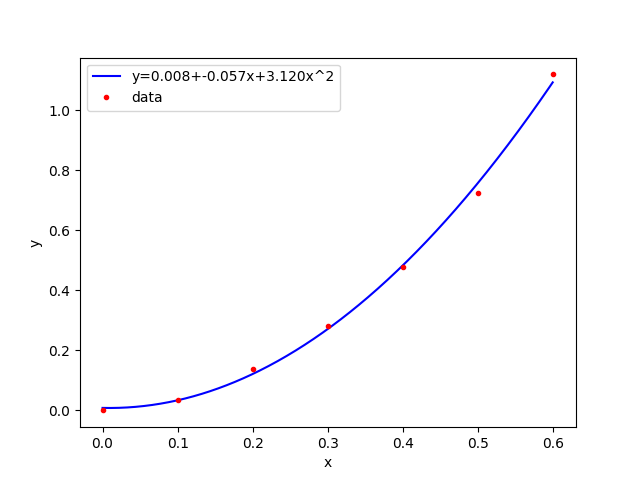
\includegraphics[width=13cm]{kadai13.png}
  \caption{課題13のグラフ}
  \label{graph11-2}
\end{figure}


\section{課題14--1 : 一次元ランダムウォーク}
\subsection{課題内容}
一次元のランダムウォークを行うプログラムを作成し、
ステップ数と分散の関係を一次と二次の最小二乗法により調査する。
また、正の方向に移動する確率$p$を変更した場合、この関係はどのように変わるのか考察する。

\subsection{プログラムリスト}
課題14--1のプログラムリストをリスト\ref{lst:kadai14-1}に示す。
課題13で作成した最小二乗法を行う関数を流用している。

\lstinputlisting[style=C,caption=課題14--1のプログラム,label=lst:kadai14-1]{code/kadai14-1.c}

\subsection{実行結果}
$p = 0.5$のときの実行結果をリスト\ref{lst:kekka14-1}に、
$p = 0.7$のときの実行結果をリスト\ref{lst:kekka14-1x}に示す。

\begin{lstlisting}[style=text,caption=pが0.5のときの実行結果,label=lst:kekka14-1]
(n, V) = ( 100,   15.523884)
(n, V) = ( 200,   32.598991)
(n, V) = ( 300,   47.586104)
(n, V) = ( 400,   61.323219)
(n, V) = ( 500,   78.533024)
(n, V) = ( 600,   98.516329)
(n, V) = ( 700,  116.542794)
(n, V) = ( 800,  131.299920)
(n, V) = ( 900,  154.414567)
(n, V) = (1000,  147.934357)
(n, V) = (1100,  189.357535)
(n, V) = (1200,  169.977783)
(n, V) = (1300,  209.623666)
(n, V) = (1400,  226.605759)
(n, V) = (1500,  253.670260)
(n, V) = (1600,  268.832560)
(n, V) = (1700,  279.689249)
(n, V) = (1800,  277.343430)
(n, V) = (1900,  345.269809)
(n, V) = (2000,  333.731190)
(n, V) = (2100,  355.947362)
(n, V) = (2200,  345.883745)
(n, V) = (2300,  421.436965)
(n, V) = (2400,  375.919495)
(n, V) = (2500,  375.621363)
(n, V) = (2600,  404.488618)
(n, V) = (2700,  431.486227)
(n, V) = (2800,  508.233071)
(n, V) = (2900,  448.499493)
(n, V) = (3000,  495.616177)
(n, V) = (3100,  514.785516)
(n, V) = (3200,  524.807244)
(n, V) = (3300,  617.592151)
(n, V) = (3400,  595.879307)
(n, V) = (3500,  519.094713)
(n, V) = (3600,  614.621791)
(n, V) = (3700,  568.387483)
(n, V) = (3800,  560.936808)
(n, V) = (3900,  695.592825)
(n, V) = (4000,  714.939175)
(n, V) = (4100,  763.579925)
(n, V) = (4200,  718.312947)
(n, V) = (4300,  626.020558)
(n, V) = (4400,  736.293271)
(n, V) = (4500,  762.235101)
(n, V) = (4600,  957.430561)
(n, V) = (4700,  785.787048)
(n, V) = (4800,  870.550813)
(n, V) = (4900,  784.626573)
(n, V) = (5000,  762.585985)

y = 0.170861x + -9.783985
y = 0.000002x^2 + 0.160822x + -1.083632
\end{lstlisting}

\begin{lstlisting}[style=text,caption=pが0.7のときの実行結果,label=lst:kekka14-1x]
(n, V) = ( 100,  148.665644)
(n, V) = ( 200,  555.972195)
(n, V) = ( 300, 1158.931700)
(n, V) = ( 400, 2180.599354)
(n, V) = ( 500, 3518.090981)
(n, V) = ( 600, 4985.400662)
(n, V) = ( 700, 6607.519793)
(n, V) = ( 800, 8601.677295)
(n, V) = ( 900, 10855.399123)
(n, V) = (1000, 14048.736173)
(n, V) = (1100, 16328.609926)
(n, V) = (1200, 19027.811397)
(n, V) = (1300, 22179.548714)
(n, V) = (1400, 26209.735436)
(n, V) = (1500, 30024.733010)
(n, V) = (1600, 34614.080243)
(n, V) = (1700, 38568.974709)
(n, V) = (1800, 43638.861840)
(n, V) = (1900, 47951.544745)
(n, V) = (2000, 53131.616736)
(n, V) = (2100, 59248.946839)
(n, V) = (2200, 64108.926276)
(n, V) = (2300, 70945.047973)
(n, V) = (2400, 78243.558186)
(n, V) = (2500, 83326.828883)
(n, V) = (2600, 89868.918849)
(n, V) = (2700, 98516.626332)
(n, V) = (2800, 104277.447543)
(n, V) = (2900, 113870.948123)
(n, V) = (3000, 121161.716834)
(n, V) = (3100, 128380.273714)
(n, V) = (3200, 137475.698790)
(n, V) = (3300, 146118.043477)
(n, V) = (3400, 153566.585019)
(n, V) = (3500, 163336.916054)
(n, V) = (3600, 175587.274039)
(n, V) = (3700, 185338.216517)
(n, V) = (3800, 193897.593360)
(n, V) = (3900, 203004.147252)
(n, V) = (4000, 215111.560730)
(n, V) = (4100, 228582.115943)
(n, V) = (4200, 236174.801135)
(n, V) = (4300, 246420.318332)
(n, V) = (4400, 257242.978548)
(n, V) = (4500, 268404.585122)
(n, V) = (4600, 283755.666438)
(n, V) = (4700, 295126.464818)
(n, V) = (4800, 309983.957599)
(n, V) = (4900, 323376.999940)
(n, V) = (5000, 332441.936831)

y = 68.286134x + -59105.009423
y = 0.013336x^2 + 0.272923x + -160.226913
\end{lstlisting}

\subsection{考察}
リスト\ref{lst:kekka14-1}の結果をプロットしたグラフを図\ref{fig:kekka14-1}、
リスト\ref{lst:kekka14-1x}の結果をプロットしたグラフを図\ref{fig:kekka14-1x}に示す。

図\ref{fig:kekka14-1}を見ると、プロットしたデータと一次の近似曲線が近い形状をしていることが分かる。
このことから、$p = 0.5$のときのステップ数と分散の関係は線形的であるといえる。

図\ref{fig:kekka14-1x}を見ると、プロットしたデータと二次の近似曲線が近い形状をしていることが分かる。
ことのこから、$p = 0.7$のときのステップ数と分散の関係は二次関数的であるといえる。

\begin{figure}[H]
  \centering
  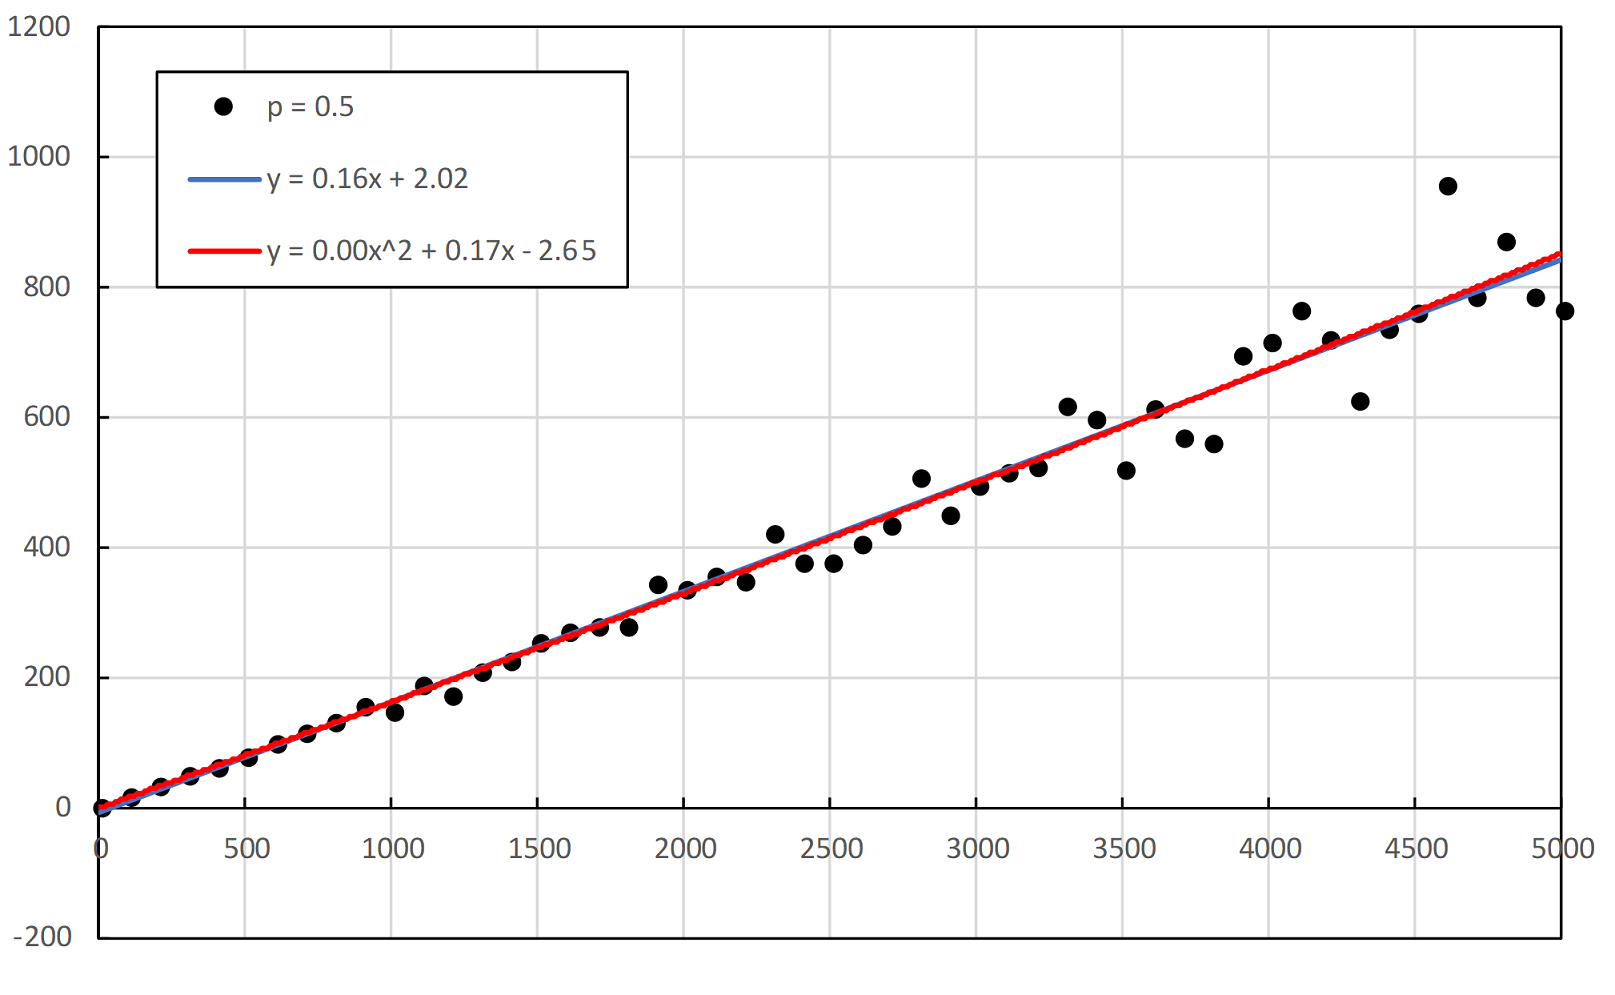
\includegraphics[width=13cm]{kadai14-1-5.png}
  \caption{$p=0.5$のときのグラフ}
  \label{fig:kekka14-1}
\end{figure}

\begin{figure}[H]
  \centering
  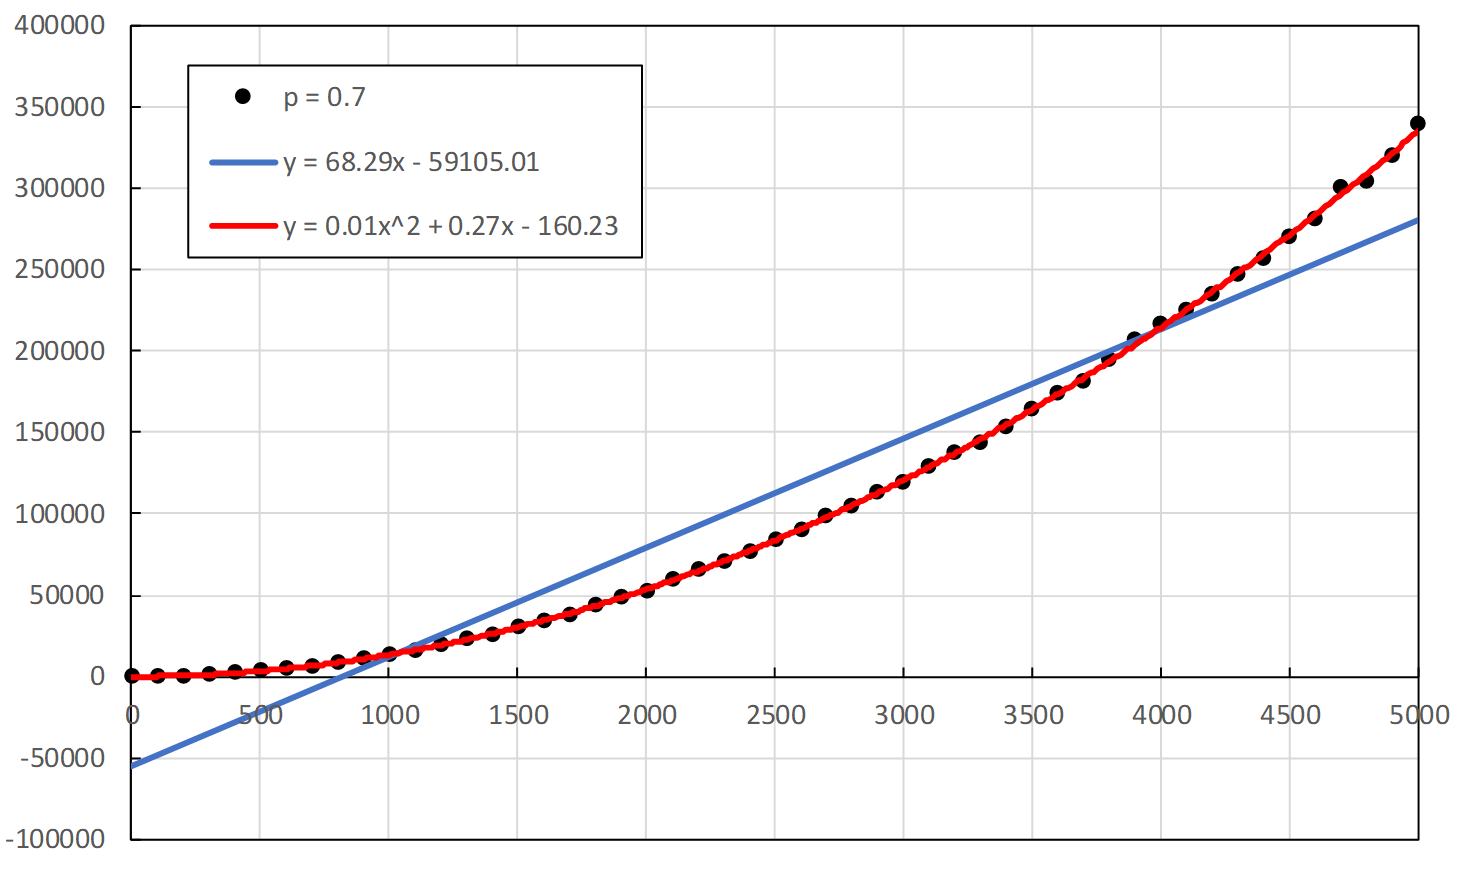
\includegraphics[width=13cm]{kadai14-1-7.png}
  \caption{$p=0.7$のときのグラフ}
  \label{fig:kekka14-1x}
\end{figure}


\section{課題14--2 : 二次元ランダムウォーク}
\subsection{課題内容}
二次元のランダムウォークを行うプログラムを作成する。
各点を1匹の蜂と見立てたとき、Nステップ後に蜂の群がどのような模様になるか調べる。

\subsection{プログラムリスト}
課題14--2のプログラムリストをリスト\ref{lst:kadai14-2}に示す。

\lstinputlisting[style=C,caption=課題14--2のプログラム,label=lst:kadai14-2]{code/kadai14-2.c}

\subsection{実行結果}
課題14-2の実行結果をリスト\ref{lst:kekka14-2}に示す。

\begin{lstlisting}[style=text,caption=課題14--2の実行結果,label=lst:kekka14-2]
(x, y) = (  8.00,  12.00)
(x, y) = (  8.00, -12.00)
(x, y) = (  0.00,  -4.00)
(x, y) = ( -2.00,  -4.00)
(x, y) = (-12.00,   0.00)
(x, y) = (  2.00,  -2.00)
(x, y) = (-12.00,   2.00)
(x, y) = ( 12.00, -12.00)
(x, y) = ( 12.00,  10.00)
(x, y) = (-28.00,  -2.00)
(x, y) = ( -6.00, -14.00)
(x, y) = (  2.00,  10.00)
(x, y) = (-20.00,  -2.00)
(x, y) = ( -4.00,  -6.00)
(x, y) = ( 14.00, -16.00)
(x, y) = ( -2.00, -20.00)
(x, y) = (  0.00, -10.00)
(x, y) = ( -2.00,   8.00)
(x, y) = (  8.00, -16.00)
(x, y) = (-18.00,  14.00)
(x, y) = (-14.00,  10.00)
(x, y) = (-16.00,  -4.00)
(x, y) = ( -4.00,  14.00)
(x, y) = (  0.00,  12.00)
(x, y) = (  0.00,   6.00)
(x, y) = ( -4.00,  -8.00)
(x, y) = ( -8.00,  -2.00)
(x, y) = ( -2.00, -10.00)
(x, y) = (-14.00,  -2.00)
(x, y) = (  4.00,  -6.00)
(x, y) = (-12.00,  10.00)
(x, y) = (  0.00,   8.00)
(x, y) = ( -6.00, -14.00)
(x, y) = ( -2.00,  14.00)
(x, y) = ( 18.00,  -2.00)
(x, y) = ( 10.00,  16.00)
(x, y) = ( -4.00,  -8.00)
(x, y) = ( 12.00, -12.00)
(x, y) = ( -2.00,  -4.00)
(x, y) = ( 22.00,   2.00)
(x, y) = (-20.00,  24.00)
(x, y) = ( -2.00,   0.00)
(x, y) = (  0.00,  -2.00)
(x, y) = (  0.00,  10.00)
(x, y) = (  4.00,  14.00)
(x, y) = ( -6.00,  18.00)
(x, y) = (  2.00,   6.00)
(x, y) = ( 10.00,  22.00)
(x, y) = ( 10.00,  -2.00)
(x, y) = ( 10.00,  -8.00)
(x, y) = ( -2.00,   2.00)
(x, y) = ( -2.00, -12.00)
(x, y) = (  6.00,  -4.00)
(x, y) = ( -8.00,   2.00)
(x, y) = ( -4.00,  -8.00)
(x, y) = ( -6.00,   8.00)
(x, y) = (  0.00,  -4.00)
(x, y) = ( -4.00, -16.00)
(x, y) = ( 16.00,  -6.00)
(x, y) = ( -4.00,   4.00)
(x, y) = (  0.00, -16.00)
(x, y) = (  2.00,   4.00)
(x, y) = (  0.00, -10.00)
(x, y) = (-24.00,   2.00)
(x, y) = (  2.00,   6.00)
(x, y) = ( 10.00,  -6.00)
(x, y) = ( -2.00,   4.00)
(x, y) = (  2.00,  14.00)
(x, y) = ( -4.00,  -8.00)
(x, y) = (-20.00,   8.00)
(x, y) = (  6.00,   4.00)
(x, y) = (-14.00,   0.00)
(x, y) = (-12.00,  -8.00)
(x, y) = (-16.00,   0.00)
(x, y) = ( -4.00,  10.00)
(x, y) = ( 12.00,  12.00)
(x, y) = ( -4.00,  20.00)
(x, y) = ( 14.00,  -6.00)
(x, y) = ( -8.00,   0.00)
(x, y) = (  0.00,   6.00)
(x, y) = ( 14.00,  -6.00)
(x, y) = (-16.00, -20.00)
(x, y) = ( 12.00,  -8.00)
(x, y) = ( 16.00,  -6.00)
(x, y) = (  4.00,  -2.00)
(x, y) = ( 12.00,  24.00)
(x, y) = (  4.00,  14.00)
(x, y) = (  0.00,  -2.00)
(x, y) = (-20.00,   6.00)
(x, y) = ( -2.00,   2.00)
(x, y) = ( -6.00, -24.00)
(x, y) = (-14.00,  -2.00)
(x, y) = (  2.00,  12.00)
(x, y) = (  0.00,  26.00)
(x, y) = ( 22.00,  12.00)
(x, y) = (  4.00,  -4.00)
(x, y) = ( -8.00,  -4.00)
(x, y) = (  4.00,   0.00)
(x, y) = ( 14.00,  14.00)
(x, y) = (  4.00,  -2.00)
(x, y) = ( -2.00,   4.00)
(x, y) = ( -6.00,   2.00)
(x, y) = (  2.00,  -2.00)
(x, y) = ( -4.00,   8.00)
(x, y) = (  2.00,  18.00)
(x, y) = (  2.00,  -4.00)
(x, y) = (  2.00,   0.00)
(x, y) = ( -4.00, -10.00)
(x, y) = ( 22.00,  14.00)
(x, y) = (-10.00,  -8.00)
(x, y) = ( 10.00,  -4.00)
(x, y) = ( -6.00,  12.00)
(x, y) = (-10.00,  -2.00)
(x, y) = (  8.00,   8.00)
(x, y) = ( -4.00,  -8.00)
(x, y) = (  0.00,   6.00)
(x, y) = (  4.00,  -4.00)
(x, y) = (  4.00,  14.00)
(x, y) = ( 10.00,   2.00)
(x, y) = ( 10.00,  10.00)
(x, y) = (-12.00,  -2.00)
(x, y) = (  4.00, -18.00)
(x, y) = ( -8.00, -20.00)
(x, y) = (-14.00,  -2.00)
(x, y) = ( -6.00,  -2.00)
(x, y) = ( 12.00,  -4.00)
(x, y) = (  4.00, -14.00)
(x, y) = ( 22.00,   8.00)
(x, y) = ( -6.00,   2.00)
(x, y) = (-10.00,  -8.00)
(x, y) = ( 16.00, -10.00)
(x, y) = ( 18.00,  -6.00)
(x, y) = (  2.00,  -8.00)
(x, y) = ( 10.00,   6.00)
(x, y) = (  2.00,   0.00)
(x, y) = (-14.00,   2.00)
(x, y) = (-10.00,  -4.00)
(x, y) = (-16.00,  -8.00)
(x, y) = ( 12.00,   4.00)
(x, y) = ( -2.00,  -6.00)
(x, y) = ( 16.00, -16.00)
(x, y) = ( 16.00,   8.00)
(x, y) = ( 12.00,  -4.00)
(x, y) = ( -2.00,  10.00)
(x, y) = ( -8.00,  16.00)
(x, y) = (  4.00,  -6.00)
(x, y) = (-12.00,  10.00)
(x, y) = (-12.00,   0.00)
(x, y) = (-14.00,   6.00)
(x, y) = (  8.00,  -8.00)
(x, y) = (-10.00,  -2.00)
(x, y) = (  6.00,   0.00)
(x, y) = ( 12.00,   4.00)
(x, y) = (  6.00, -18.00)
(x, y) = ( 12.00, -18.00)
(x, y) = (  0.00, -16.00)
(x, y) = (-28.00,   8.00)
(x, y) = ( -4.00,  -8.00)
(x, y) = (  4.00,   6.00)
(x, y) = (  8.00,  -2.00)
(x, y) = ( -6.00,  -6.00)
(x, y) = (  4.00,  12.00)
(x, y) = (  6.00,   6.00)
(x, y) = ( -6.00,  26.00)
(x, y) = ( 14.00,   2.00)
(x, y) = (  4.00,   2.00)
(x, y) = ( -8.00,   8.00)
(x, y) = ( -6.00,  -2.00)
(x, y) = ( -4.00,  -2.00)
(x, y) = (-28.00,  10.00)
(x, y) = (-10.00, -10.00)
(x, y) = ( -8.00,   0.00)
(x, y) = (  4.00,  26.00)
(x, y) = ( -4.00,  -8.00)
(x, y) = (  4.00, -16.00)
(x, y) = (-14.00,   6.00)
(x, y) = ( 14.00,   2.00)
(x, y) = (  0.00,   8.00)
(x, y) = ( 10.00,  -6.00)
(x, y) = ( -2.00,  -8.00)
(x, y) = ( -4.00,  -6.00)
(x, y) = (  2.00,   8.00)
(x, y) = ( -2.00,   4.00)
(x, y) = (-18.00,  -4.00)
(x, y) = ( -6.00, -12.00)
(x, y) = ( 14.00,   0.00)
(x, y) = (  2.00,  10.00)
(x, y) = (-14.00,   0.00)
(x, y) = ( 12.00,   6.00)
(x, y) = ( -8.00,  -2.00)
(x, y) = (-12.00,   8.00)
(x, y) = (-12.00,   0.00)
(x, y) = (-10.00,  -4.00)
(x, y) = (  4.00,  -4.00)
(x, y) = ( 14.00,  10.00)
(x, y) = ( -2.00,   2.00)
(x, y) = (-12.00,  -6.00)
(x, y) = ( -2.00,   8.00)
(x, y) = ( -2.00,   0.00)
(x, y) = ( -4.00, -12.00)
\end{lstlisting}

\subsection{考察}
$N=$100, 1000, 10000のときの結果をプロットしたグラフを図\ref{fig:100}, \ref{fig:1000}, \ref{fig:10000}に示す。

図\ref{fig:100}--\ref{fig:10000}を見ると、$N$の値が大きくなればなるほど、群のばらつきが大きくなることが分かる。
これは課題14--1の結果からも分かるように、ステップ数が多くなればなるほど、分散すなわちばらつきが大きくなるからと考えられる。

\begin{figure}[H]
  \centering
  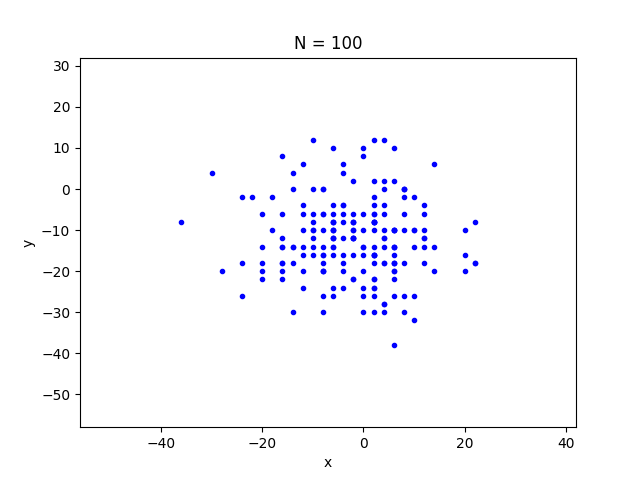
\includegraphics[width=13cm]{n100.png}
  \caption{$N = 100$}
  \label{fig:100}
\end{figure}

\begin{figure}[H]
  \centering
  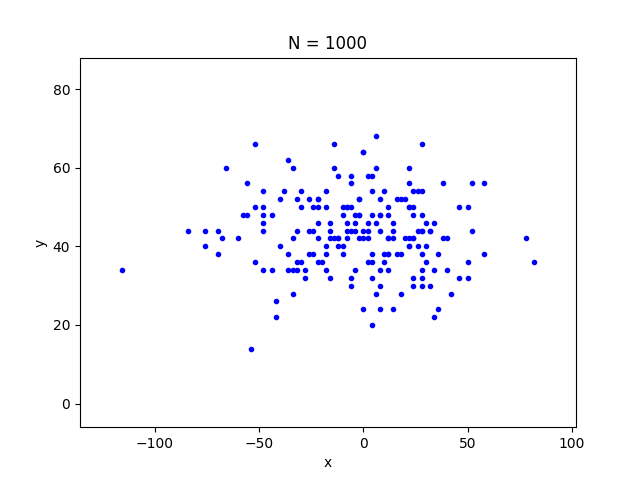
\includegraphics[width=13cm]{n1000.png}
  \caption{$N = 1000$}
  \label{fig:1000}
\end{figure}

\begin{figure}[H]
  \centering
  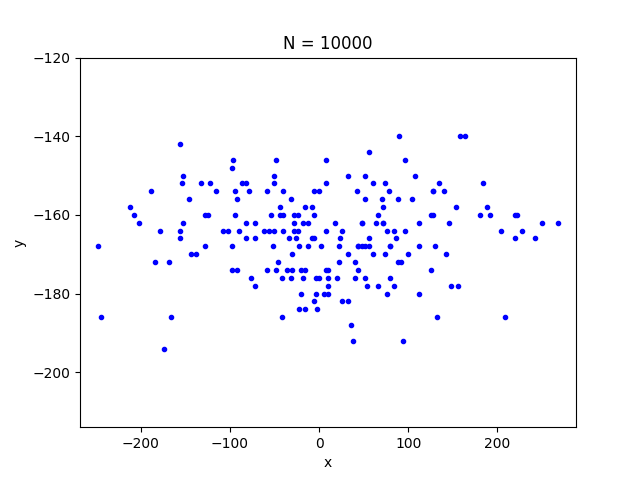
\includegraphics[width=13cm]{n10000.png}
  \caption{$N = 10000$}
  \label{fig:10000}
\end{figure}


\end{document}
